
\documentclass[11pt]{article}

\usepackage{common}
\title{HW1: Text Classification}
\author{Rohil Prasad \\ prasad01@college.harvard.edu \and Jeffrey Ling \\ jling@college.harvard.edu }
\begin{document}

\maketitle{}
\section{Introduction}

Text classification and sentiment analysis is an old problem with applications ranging from business analytics to finance.
It is an easy task for humans to tell whether a piece of writing pertaining to some topic speaks positively or negatively about that topic. 
For example, we know immediately that a movie review containing the phrase ``worst movie ever'' is extremely negative, while the opposite phrase 
``best movie ever'' indicates an extremely positive review. We are also capable of easily parsing more high-level semantic features such as context and sarcasm.

This problem is much more difficult for a computer that cannot naively detect things such as context and sarcasm. However, we can construct supervised learning algorithms that 
can be used to train good estimators of text sentiment. 

In this paper, we explore three methods of classifying the sentiment of movie reviews from the Stanford Sentiment database. These three methods are multinomial naive Bayes, 
logistic regression with L2 regularization, and hinge-loss linear SVM with L2 regularization. 

In Section $2$, we introduce our notation and give a description of our problem in formal language. In Section $3$, we describe our three algorithms as implementations of 
the probabilistic linear model. In Section $4$, we present our experimental results for hyperparameter tuning and algorithm performance. In Section $5$, we conclude with a 
discussion of our results. 

\section{Problem Description}

We arrange the training data into pairs $x_i, y_i$ for $i = 1, \ldots, N$. For brevity we call each data point $x, y$, where $x$ is a sentence and $y \in \mcY$ is the sentiment class of the sentence, and $\mcY$ is a finite set.

We represent $x$ by its features $x \in \{0, 1\}^f$. In this homework, we featurize a sentence as a bag of unigrams, i.e. a feature $x_j = 1$ iff the word corresponding to index $j$ is in the sentence. The index $j$ indexes into the vocabulary $\mcV$ of the training and testing dataset.

Our goal is to predict the correct class $c$ by learning a function $f : \{0, 1\}^f \to \mcY$, where $\widehat{y}_k = f(x)$ is the predicted probability $p(k | x)$ of $x$ belonging to class $k$. We will do this through some linear models.

%In general, homeworks will be specified using informal
%language. As part of the assignment, we expect you to write-out a
%definition of the problem and your model in formal language. For this
%class, we will use the following notation:
%
%\begin{itemize}
%\item $\boldb, \boldm$;  bold letters for vectors.
%\item $\boldB, \boldM$;  bold capital letters for matrices.
%\item $\mcB, \mcM$;  script-case for sets.
%\item $b_i, x_i$; lower case for scalars or indexing into vectors.
%\end{itemize}
%
%
%For instance in natural language processing, it is common to use
%discrete sets like $\mcV$ for the vocabulary of the language, or $\mcT$ for a
%tag set of the language.  We might also want one-hot vectors
%representing words. These will be of the type
%$\boldv \in \{0,1\}^{|\mcV|}$. In a note, it is crucial to define the
%types of all variables that are introduced. The problem description is the
%right place to do this.

% NLP is also
% full of sequences. For instance sentences, $w_1, \ldots, w_N$, where
% here $N$ is a constant length and $w_i \in \mcV$ for all
% $i \in \{1, \ldots N\}$. If we pretend sentences are all the same
% length, we can have scoring function over sentences,
% $s : \mcV^N \mapsto \reals$.  One might be defined as:

% \[ s(w_1, \ldots, w_N) = \sum_{i = 1}^N p(w_i | w_{i-2}, w_{i-1}), \]

% \noindent where $p$ is the bigram probability, which we will cover later in the class.

\section{Model and Algorithms}

We use three models in this experiment:

\begin{enumerate}
\item multinomial naive Bayes (MNB)
\item logistic regression with L2 regularization
\item hinge-loss linear SVM with L2 regularization 
\end{enumerate}

We describe the setup of each.

\subsection{Multinomial Naive Bayes}

In MNB, we assume that the features of $x$ are independent of each other. Specifically, in order to obtain $p(y | x)$, the probability of class $y$ given input $x$, we apply Bayes rule to get
$$p(y | x) = \frac{p(x | y)p(y)}{p(x)}$$
or in log space,
$$\log p(y | x) = \log p(x | y) + \log p(y) - \log p(x)$$
with prediction given by
$$\widehat{y} = \argmax_y p(y|x)$$
Since $p(x)$ is a constant function of $y$, we can omit it from our predictor, so it suffices to learn $p(x | y)$ and $p(y)$.

If $x$ is represented as binary features $x_1, \ldots, x_k$, then under the independence assumption we have
$$p(x | y) = p(x_1, \ldots, x_k | y) = p(x_1 | y) \cdots p(x_k | y)$$
The parameters are thus $p(x_f | y)$, which under negative log-likelihood loss, is maximized over the training data by counting the number of samples with $x_f$ in class $y$ and dividing by the total number of samples from class $y$.

Similarly, the MLE estimate of $p(y)$ is the proportion of training samples that are of class $y$. Thus, our prediction is
$$\widehat{y} = \argmax_y \sum_i \log p(x_i | y) + \log p(y)$$

The sum is taken over features that appear in $x$. Note that this has the form of a linear model with linear weights $W$ as the $\log p(x_i | y)$ and intercept $b$ as $\log p(y)$.

In our task, if we write $x$ in its sparse feature representation with each feature being an indicator of a word, we can write $\widehat{y} = xW + b$.

\subsection{Logistic Regression}

In logistic regression, we assume $z = xW + b$, where $x$ is the feature representation of the data point. We then perform the softmax function to obtain $\widehat{y_i} = e^{z_i} / \sum_{z'} e^{z'}$ which gives $\widehat{y_i} = p(y_i | x)$.

Our criterion function here is the negative log-likelihood loss, plus a regularization term:
$$L(X, Y; W, b) = \sum_x -\log \widehat{y}_c + \frac{\lambda}{2} {\lVert W \rVert}^2$$
where $\widehat{y}_c$ is the predicted probability for the correct class $c$ for a given $x$. $\lambda$ is a hyperparameter that can be tuned.

We optimize the loss over the training set with gradient descent. We have that
$$\frac{\partial L}{\partial W_{i,j}} = x_j \frac{\partial L}{\partial z_i}, \frac{\partial L}{\partial b_i} = \frac{\partial L}{\partial z_i}$$
where $\partial L / \partial z_i$ equals the predicted $\widehat{y_i}$ under softmax, except $\partial L / \partial z_c = \widehat{y_c} - 1$.

We perform minibatch gradient descent with batch size a tunable hyperparameter. For each batch, we take the average gradient of the samples in the batch. Each gradient descent step is a combination of regularization shrinkage and subtracting of the computed gradient:
$$\theta \leftarrow (1 - \eta \lambda m / N) \theta - \eta \mathbf{g}$$
where $\mathbf{g}$ is the computed gradient, $m$ is the batch size, and $N$ is the number of training points.

For the batches, we shuffle the training data once, then iterate through it one batch at a time. One sweep of the entire data is a single epoch. We picked a stopping criterion as
$$\frac{| loss - prevLoss |}{prevLoss} < 0.001$$
where the losses are computed over the validation set at the end of each epoch.

\subsection{Hinge-loss Linear SVM}

The hinge loss model is exactly the same as logistic regression, except instead of negative log likelihood loss, we use the hinge loss, defined as
$$L(y, \widehat{y}) = \max(0, 1 - (\widehat{y}_c - \widehat{y}_{c'}))$$
where $c$ is the correct class and $c' = \argmax_{c' \neq c} \widehat{y}_{c'}$.

So our overall criterion is
$$L(X, Y; W, b) = \sum_x \max(0, 1 - (\widehat{y}_c - \widehat{y}_{c'})) + \frac{\lambda}{2} \lVert W \rVert ^2$$

The gradients in this case have the same form as in logistic regression, except $\partial L / \partial z_i$ changes. We compute these to be:
$$\frac{\partial L}{\partial z_i} = \begin{cases} 0 \indent \widehat{y}_c - \widehat{y}_{c'} > 1 \\
 \widehat{y}_i(\widehat{y}_c - \widehat{y}_{c'}) - \widehat{y}_c \indent i = c \\
\widehat{y}_i(\widehat{y}_c - \widehat{y}_{c'}) + \widehat{y}_{c'} \indent i = c' \\
\widehat{y}_i(\widehat{y}_c - \widehat{y}_{c'}) \indent else \end{cases}$$

The gradient descent method is the same as before.


\begin{figure}

  \begin{algorithmic}[1]
    \Procedure{GradientDescent}{$\{ X_i \}$,  $\{ y_i \} $}
	\State{$W, b \gets 0$}
	\While{stopping condition not met}
		\State{randomly sample batch of size $m$}
		\State{$\mathbf{g_W} \gets \partial L / \partial W_{ij}$}
		\State{$\mathbf{g_b} \gets \partial L / \partial b$}
		\State{$W \gets (1 - \eta \lambda m / N) W - \eta \mathbf{g_W}$}
		\State{$b \gets b - \eta \mathbf{g_b}$}

    \EndWhile{}
    \State{\Return{$W, b$}}
    \EndProcedure{}
  \end{algorithmic}

\end{figure}


\section{Experiments}

We ran several hyperparameter settings on SST1 and discovered the following optimal settings for each model: for MNB, $\alpha = 1.0$; for logistic regression, $\eta = 0.1, \lambda = 1.0$; for hinge loss, $\eta = 0.1, \lambda = 0.1$. We used batch size of 50 and ran for a maximum of 50 epochs for all experiments.

With these hyperparameters, we run experiments on the validation sets of SST1 and SST2 and report the percentage of samples predicted correctly. We implement 10-fold cross validation on MPQA and Subj (which do not come with validation sets) to find the average performance over folds. Note that SST1 has 5 classes, while other datasets are binary.

\begin{table}[h]
\centering
\begin{tabular}{llccccc}
 \toprule
 Model &  & SST1 & SST2 & MPQA & Subj & TREC \\
 \midrule
 \textsc{MNB} & & 39.9 & 80.6 & 83.8 & 92.2 & 76.4\\
 \textsc{Logistic} & & 39.2 & 78.9 & 71.0 & 87.9 & 68.2 \\
 \textsc{Linear SVM} & & 37.6  & 70.4 & 68.3 & 84.3 & 50.4 \\
 \bottomrule
\end{tabular}
\caption{\label{tab:results} Results with optimal hyperparameters.}
\end{table}

These results are slightly worse than the baselines reported in Wang and Manning (2012). For naive Bayes, we hypothesize that our shuffling of data in cross-validation may have affected the performance. For regression, this is probably because we did not have time to run gradient descent to its full optimum, and we also may have used different batch sizes in gradient descent.

% Timing

We also kept track of the training time for each algorithm to make sure that everything was running at a feasible speed. The times for the logistic regression and linear SVM are taken as an average per epoch. 

\begin{table}[h]
  \centering
  \begin{tabular}{llc}
    \toprule
    Model & & Time (s) \\
    \midrule
    \textsc{MNB} & & 2 \\
    \textsc{Logistic} & & 20 \\
    \textsc{Linear SVM} & & 19 \\
  \end{tabular}
  \caption{\label{tab:timing} Training time estimates.}
\end{table}

As expected, naive Bayes is the fastest by far since it has a closed form solution. The other two algorithms required gradient descent. Although we optimized the gradient calculation with Torch, there is still a noticeable difference. 

We also kept track of loss via console output to make sure that our algorithms were training properly. The diagram below is a plotting of one of our test runs for linear SVM with $\eta = 0.1$ and $\lambda = 0.01$. 

\begin{figure}
  \centering
  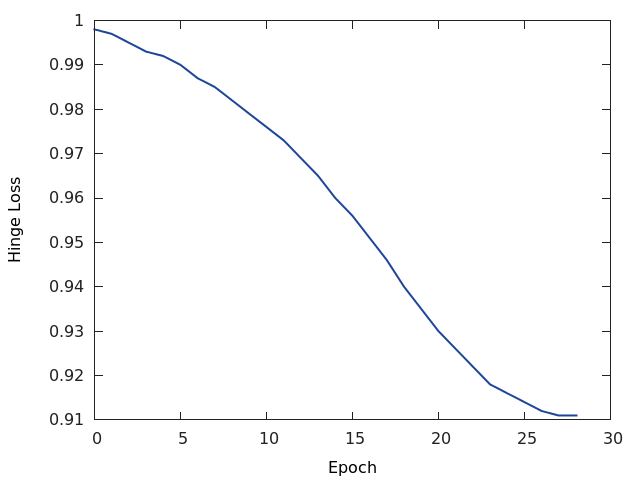
\includegraphics[width=6cm]{hinge}
  \caption{\label{fig:loss} Loss curve for linear SVM}
\end{figure}

% Gradient descent is working curves
%%\begin{figure}
%  \centering
%  \includegraphics[width=6cm]{cluster_viz}
%  \caption{\label{fig:clusters} Sample qualitative chart.}
%\end{figure}


\section{Conclusion}

%End the write-up with a very short recap of the main experiments and the main results. Describe any challenges you may have faced, and what could have been improved in the model.

In this homework we implemented basic linear models for text classification. We almost achieved several baselines, though our implementation was slightly worse in performance.

One challenge we ran into was debugging gradient descent. In order to troubleshoot our models, computing numerical gradients turned out to be extremely helpful in discovering where our gradients were being computed incorrectly. We recommend that any gradient-based method come with a test to ensure that gradients are being computed correctly.

Another challenge we ran into was tuning hyperparameters. Although we tried to get training time down as much as we could, logistic regression and linear SVM took too long to do an extensive grid search. Luckily, we were able to find some good values without too many trials. 

\bibliographystyle{apalike}
\bibliography{writeup}
Wang, Sida, and Christopher D. Manning. "Baselines and bigrams: Simple, good sentiment and topic classification." Proceedings of the 50th Annual Meeting of the Association for Computational Linguistics: Short Papers-Volume 2. Association for Computational Linguistics, 2012.

\end{document}
